\chapter{Legislação}
\label{ch:identificador}

\section{Normas para o uso de drone no Brasil}

Segundo a Norma ICA 100 - 40 \cite{(ICA100)} e a RBAC-E Nº 94 EMENDA Nº 03 \cite{(RBAC-E)} para os drones da empresa Drop Flash operarem é necessário seguir a risca as seguintes regras de voo:\\

RPA de peso máximo de decolagem superior a 250g e até 25kg (classe 3) - Em VLOS de 40m até 120m acima do nível do solo. 

\begin{enumerate}
    \item Ter idade igual ou superior a 18 anos para pilotar;
    \item Serão obrigatórias licença e habilitação emitidas pela ANAC (Agência Nacional de Aviação Civil);
    \item Registro emitido junto à ANAC e sua identificação na aeronave; (Obteremos uma aeronave já cadastrada na ANAC).
    \item Apólice de seguro ou certificado de seguro com comprovante de pagamento com cobertura de danos a terceiros (seguro reta);
    \item Documento que contém a avaliação de risco operacional elaborada pelo operador conforme E-94-003 da ANAC; (E-94-003 tem o modelo, instruções e exemplos de como fazer a avaliação de risco operacional).
    \item Manual completo do drone;
    \item Certificado de homologação na ANATEL (Agência Nacional de Telecomunicações) ou número de homologação na ANATEL gravado na aeronave;(obteremos um drone já homologado).
    \item Autorização de voo emitida pelo DECEA (Departamento de Controle do Espaço Aéreo); (Solicitação de voo pelo sistema SARPAS, tempo para aprovação é de 45 minutos, para solicitar voo é necessário o registro emitido pela ANAC e a homologação na ANATEL. Serviço gratuito).
    \item Conhecer os meios de contato do órgão regional responsável pela área de operação;
    \item Conhecer os meios de contato com o órgão ATS mais próximo da área de operação; (Órgão ATS “órgão dos serviços de tráfegos”, ou seja, DECEA e seus subordinados).
    \item Operar em condições VMC; (Condições meteorológicas, expressas em termos de visibilidade, distância de nuvens e teto, iguais ou superiores aos mínimos especificados para o voo visual. Esses mínimos, em princípio, exigem teto de 450 metros e visibilidade igual ou superior a 5 quilômetros, embora outros valores possam ser aplicáveis, conforme a situação do voo pretendido).
    
    \begin{figure} [!ht]
       {\centering
        \caption{Mínimo de visibilidade e distância de nuvens em VMC}
        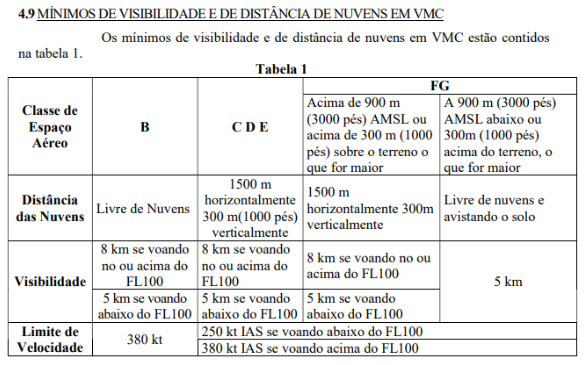
\includegraphics[width=0.9\linewidth]{figuras/vms.png}
        \label{fig:enter-label}
        \fonte{DACEA}
        }
    \end{figure}

\item Velocidade máxima de 120 km/h; 
    \item Altura de voo máxima de 120m; 
    \item Não requer comunicação bilateral com órgão ATS se estiver operando dentro dos limites estabelecidos; 
    \item Realizar operação VLOS, em área circular, polígono ou corredor, sendo limitada a uma distância horizontal que permita a manutenção da visualização da aeronave, com ou sem auxílio de um ou mais observadores; (Operação na qual o piloto, sem o auxílio de observadores de RPA, mantém o contato visual direto (sem auxílio de lentes ou outros equipamentos) com a aeronave remotamente pilotada, de modo a conduzir o voo com as responsabilidades de manter as separações previstas com outras aeronaves, bem como de evitar colisões com aeronaves e obstáculos”. Essa é a forma mais comum de se utilizar o drone, manter na linha de visada do piloto é uma forma que aumenta em muito a segurança).
    \item Afastamento mínimo de 30 m de pessoas não anuentes, animais e propriedades de terceiros com exceção dos órgãos de segurança pública;
    \item Afastamento mínimo de 9 km aeródromos cadastrados, quando operando nas zonas de aproximação e de decolagem;  
    \item Afastamento mínimo de 3 km do centro de helipontos cadastrados independente da altura do heliponto;
    \item Afastamento mínimo de 2 km de áreas nas quais sejam previstas operações ligadas à aviação agrícola.     
\end{enumerate}


\section{Liberação da empresa}

Para o funcionamento da empresa Drop Flash é necessário:\\

\textbf{Alvará de funcionamento (AFL)}
O Auto de Licença de Funcionamento (ALF) é o documento obrigatório que autoriza o funcionamento de atividades que não são residenciais, como comércios, indústrias ou serviços.\\

\textbf{Alvará de localização}
Para que a Drop Flash seja inaugurada no Brasil, é necessário verificar se o local onde o negócio será implantado está disponível. A inspeção técnica realizada pelo fiscal municipal é obrigatória.\\

\textbf{Licença prévia }
Durante o planejamento inicial, é possível solicitar uma Licença Prévia, para modificar ou expandir a estrutura de um estabelecimento. Este tipo de autorização garante que a empresa está em conformidade com os padrões ambientais necessários para a construção do negócio.\\

\textbf{Licença de instalação} 
A licença de instalação confirma que o projeto está em conformidade com as leis atuais e permite legalmente o início das obras no terreno.\\

\textbf{Licença de operação}
A obtenção de uma licença de operação é crucial para iniciar as operações do empreendimento. Quando emitida, indica que a empresa cumpriu os requisitos fundamentais e obrigatórios estabelecidos por lei para o planejamento, instalação e funcionamento do seu negócio.\\
